% EXPERIMENTO 1
\subsection{Experimento 1: sustitución de la función REF por la función de Dombi en el algoritmo de maximización de la similitud}
\subsubsection{Explicación del experimento}
En este primer experimento pretendemos conocer cómo se pueden adaptar las funciones de Dombi que hemos descrito en \ref{def:dombi} para la sustitución de las funciones REF en la creación de los conjuntos difusos. Para ello, se tomarán las imágenes que se muestran en la figura \ref{fig:imagenesexp1dombi} junto con sus hitogramas así como las imágenes ya umbralizadas por parte de un experto. 

En primer lugar, se procesarán las imágenes para conocer la forma de sustitución con $w=1$ tanto para $x$ como para $y$. Después, y a la vista de unos resultados variables, se toma la determinación de ampliar el rango de pesos por lo que se prepara una prueba para los valores 0,1; 0,5; 0,75; 1; 1,25; 1,5; 2 y 5. Por último, para poder conocer la efectividad de todos estos resultados, son comparados contra el algoritmo de maximización de la similitud original tomando como equivalencia restringida todas las funciones que se han enumerado anteriormente en \ref{obs:funcionesref}, dándole especial importancia a la $REF(x,y)=1-\abs{x-y}$ así como con todos los demás algoritmos explicados en el apartado \ref{sec:otrosalgoritmos} de la sección anterior. 

Para poder conocer de forma empírica la diferencia entre dos imagenes segmentadas, se calcula para todas ellas el error cuadrático medio. Se puede expresar el error como
$$ECM(Q, Q') = \frac{\sum_{x=1}^N\sum_{y=1}^M \left(q(x,y)-q'(x,y)\right)^2}{N\cdot M}.$$

Para poder conocer cómo actua el algoritmo frente al ruido, se han preparado imágenes con ruido gausiano con media $\mu=0$ y varianza $\sigma^2 = 0,01$. También, se han preparado con ruido impulsivo, de `de sal y pimienta' con densidad de probabilidad del ruido $d=0,05$ y $d=0,2$. Se presentan las imágenes ya tratadas en la figura \ref{fig:sillaconruido}. Por otra parte, se prueba a ver cómo resiste el algoritmo con imágenes de bajo y alto contraste. Se pueden ver en la figura \ref{fig:sillaconcontraste}.

\begin{figure}
\centering
    \subfigure[`Silla']
    {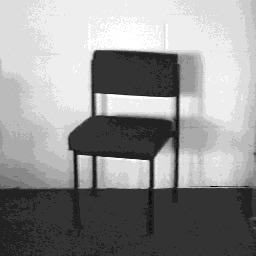
\includegraphics[width=0.22\textwidth]{img/orig/chair.jpg}}\quad
    \subfigure[Histograma]
    {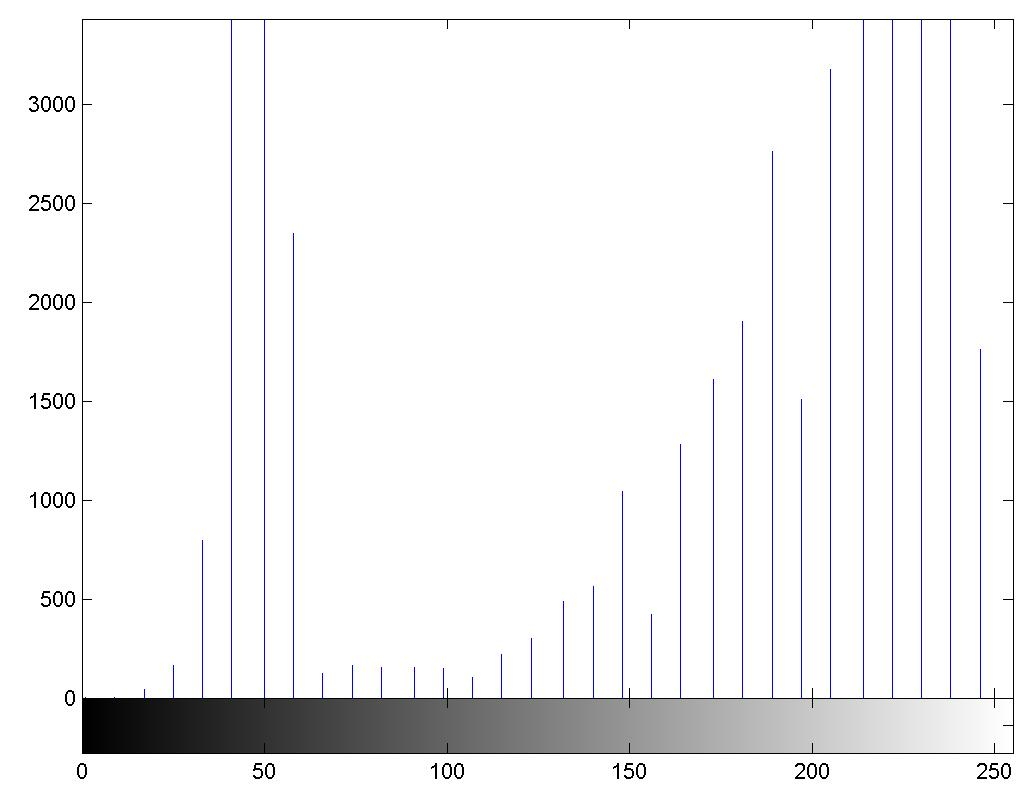
\includegraphics[width=0.28\textwidth]{img/hist/hist-chair.jpg}}\\
    \subfigure[`Bloques']    
    {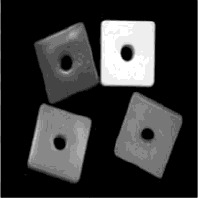
\includegraphics[width=0.22\textwidth]{img/orig/block.jpg}}\quad
    \subfigure[Umbralización del experto.]
    {
\includegraphics[width=0.22\textwidth]{img/orig/blockbin.jpg}}\quad
    \subfigure[Histrograma]
    {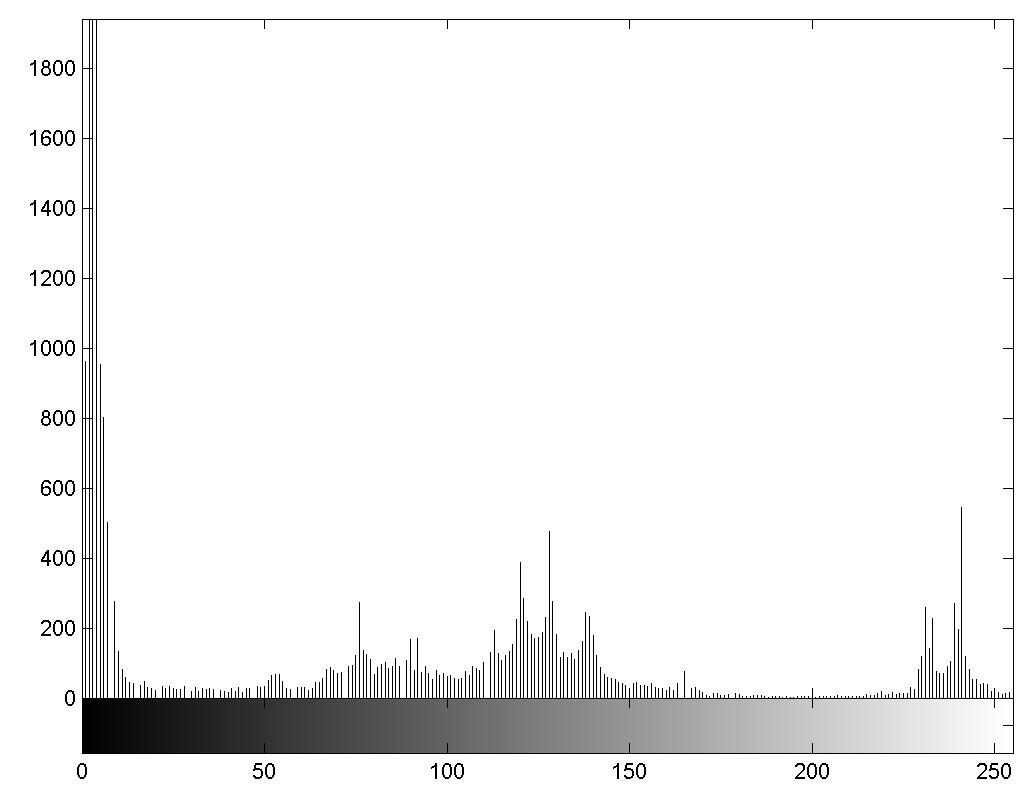
\includegraphics[width=0.28\textwidth]{img/hist/hist-block.jpg}}\\
    \subfigure[`Engranaje']
    {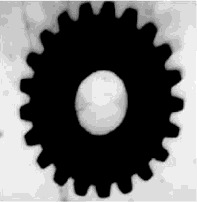
\includegraphics[width=0.22\textwidth]{img/orig/02.jpg}}\quad
    \subfigure[Umbralización del experto.]
    {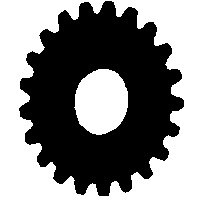
\includegraphics[width=0.22\textwidth]{img/orig/02bin.jpg}}\quad
    \subfigure[Histrograma]
    {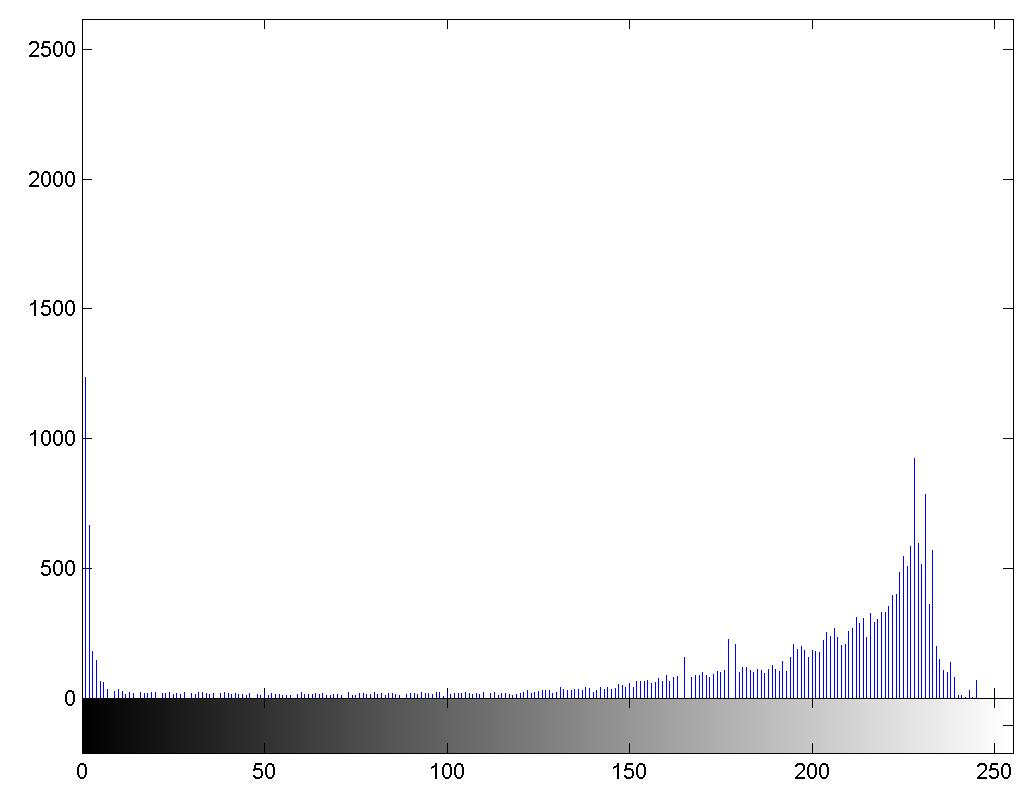
\includegraphics[width=0.28\textwidth]{img/hist/hist-02.jpg}}\\
    %\subfigure[`Piedras']
    %{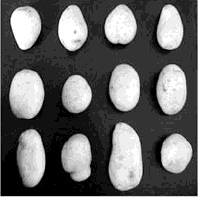
\includegraphics[width=0.22\textwidth]{img/orig/04.jpg}}\quad
    %\subfigure[Umbralización del experto.]
    %{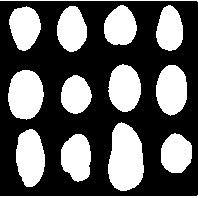
\includegraphics[width=0.22\textwidth]{img/orig/04bin.jpg}}\quad
    %\subfigure[Histrograma]
    %{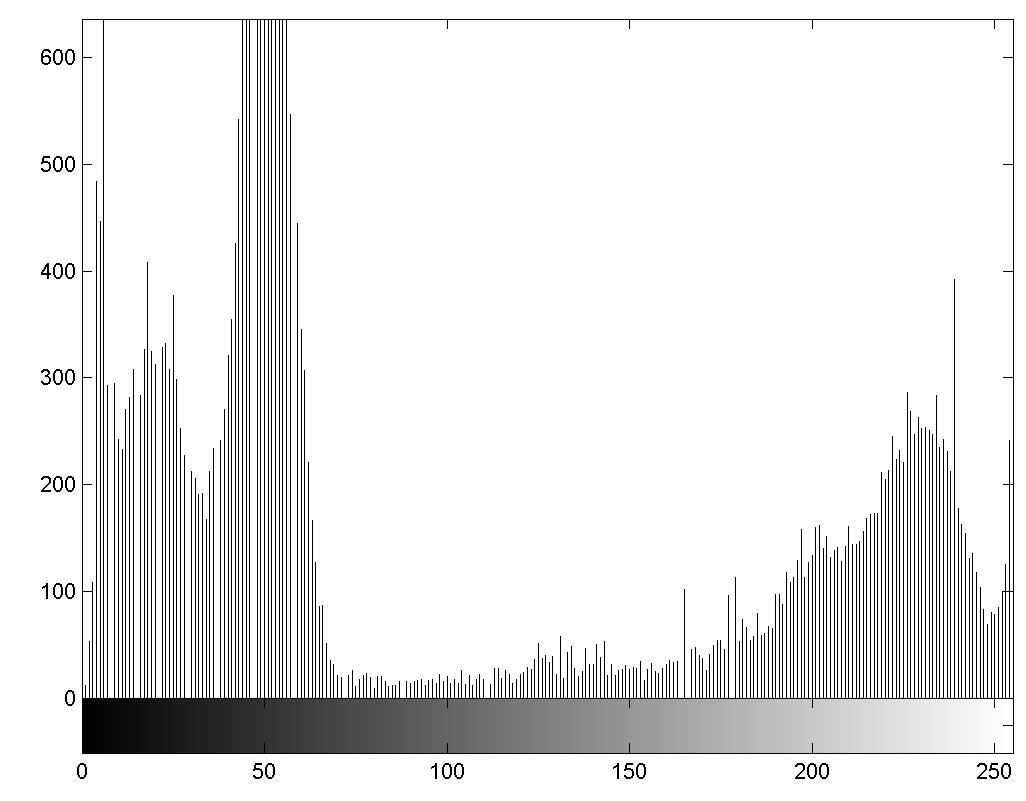
\includegraphics[width=0.28\textwidth]{img/hist/hist-04.jpg}}\\
    \subfigure[`Letras']
    {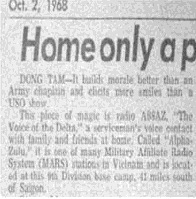
\includegraphics[width=0.22\textwidth]{img/orig/09.jpg}}\quad
    \subfigure[Umbralización del experto.]
    {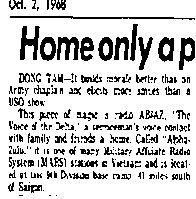
\includegraphics[width=0.22\textwidth]{img/orig/09bin.jpg}}\quad
    \subfigure[Histrograma]
    {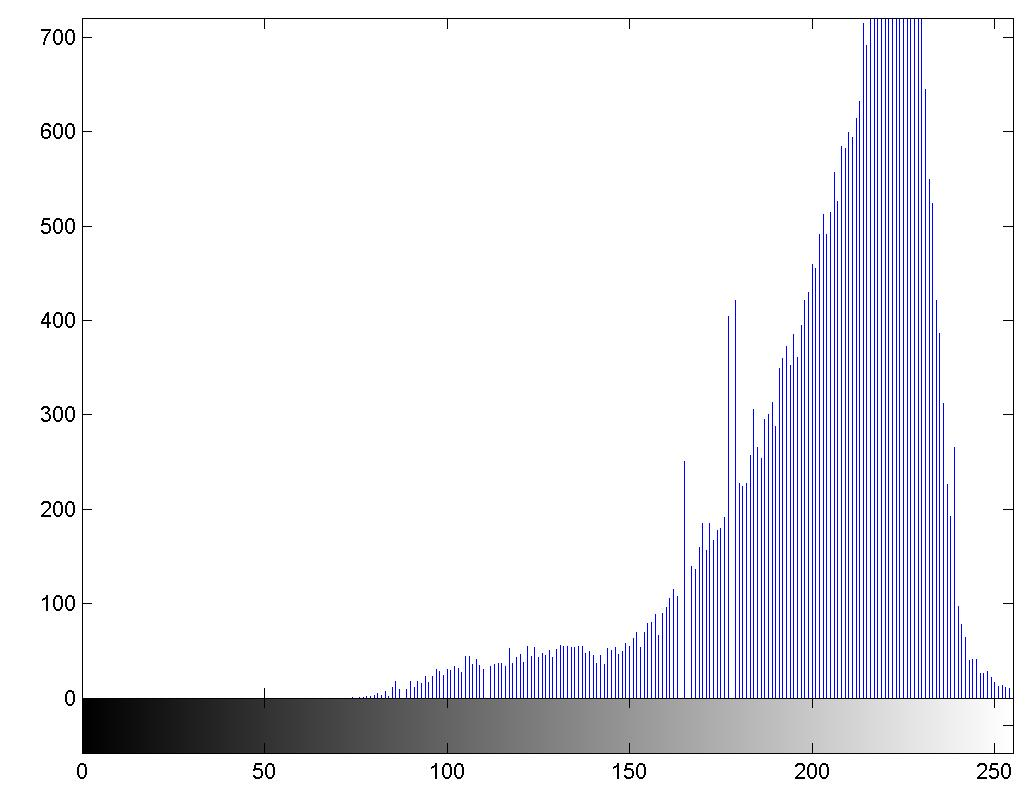
\includegraphics[width=0.28\textwidth]{img/hist/hist-09.jpg}}
    \subfigure[`Sombra']
    {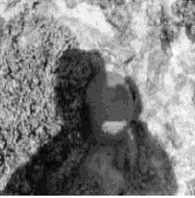
\includegraphics[width=0.22\textwidth]{img/orig/07.jpg}}\quad
    \subfigure[Umbralización del experto.]
    {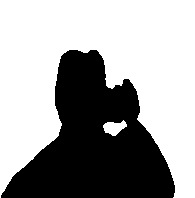
\includegraphics[width=0.22\textwidth]{img/orig/07bin.jpg}}\quad
    \subfigure[Histrograma]
    {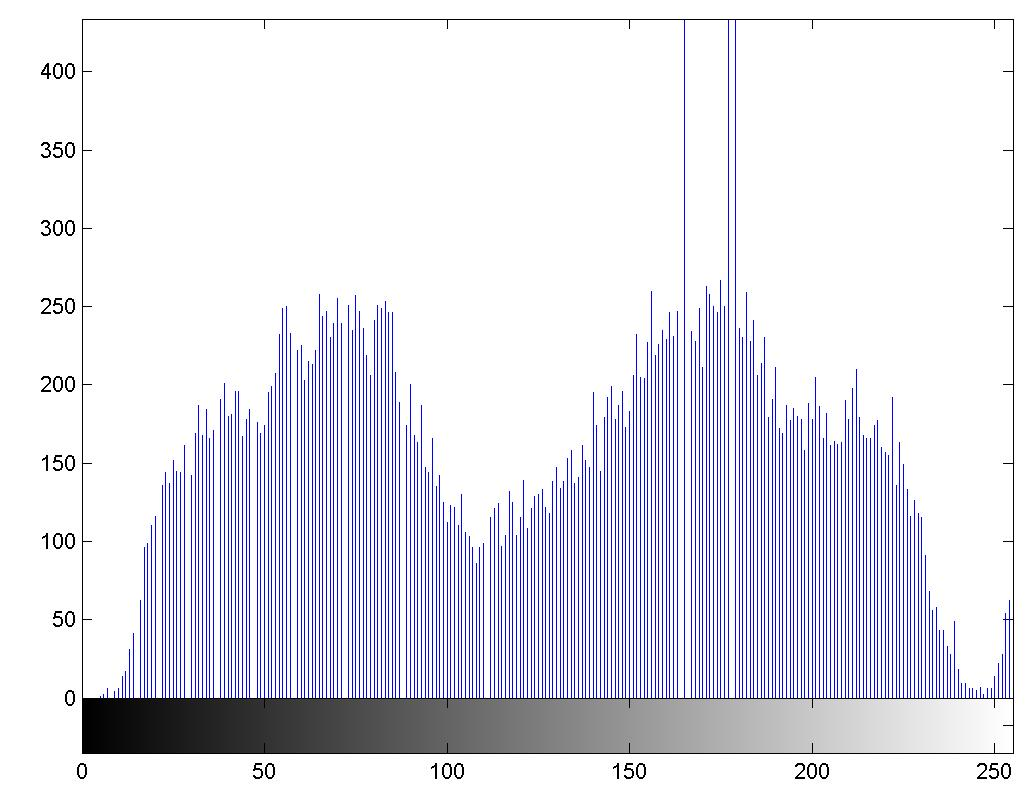
\includegraphics[width=0.28\textwidth]{img/hist/hist-07.jpg}}
    \caption{Imágenes utilizadas en el experimento 1 y siguientes.}
    \label{fig:imagenesexp1dombi}
\end{figure}

\begin{figure}
\centering
    \subfigure[Ruido gausiano]
    {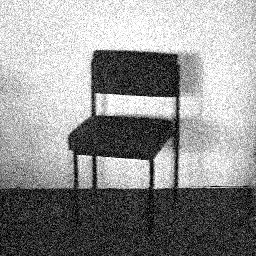
\includegraphics[width=0.25\textwidth]{img/orig/chairga.jpg}}\quad
    \subfigure[Ruido `sal y pimienta' con $d=0,05$]
    {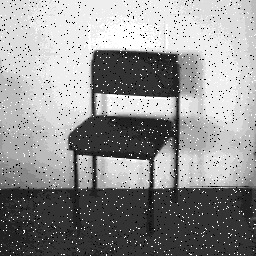
\includegraphics[width=0.25\textwidth]{img/orig/chairs&p005.jpg}}\quad
    \subfigure[Ruido `sal y pimienta' con $d=0,2$]    
    {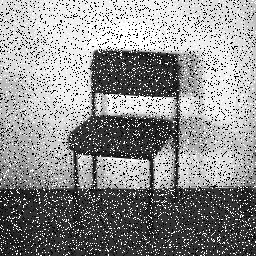
\includegraphics[width=0.25\textwidth]{img/orig/chairs&p020.jpg}}
    \caption{Imágenes con ruido utilizadas en el experimento 1 y siguientes.}
    \label{fig:sillaconruido}
\end{figure}

%\REV{incluir figura}
%\begin{figure}
%\centering
%    \subfigure[Muy alto contraste]
%    {\includegraphics[width=0.22\textwidth]{img/orig/chairmuyacon.jpg}}\quad
%    \subfigure[Alto contraste]
%    {\includegraphics[width=0.22\textwidth]{img/orig/chairacon.jpg}}\quad
%    \subfigure[Bajo contraste]
%    {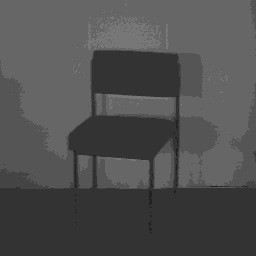
\includegraphics[width=0.22\textwidth]{img/orig/chairbcon.jpg}}\quad
%    \subfigure[Muy bajo contraste]    
%    {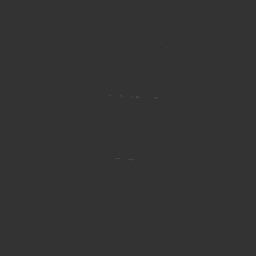
\includegraphics[width=0.22\textwidth]{img/orig/chairmuybcon.jpg}}
%    \caption{Imágenes con ruido utilizadas en el experimento 1 y siguientes.}
%    \label{fig:sillaconcontraste}
%\end{figure}

\subsubsection{Resultados}
En la figura \ref{fig:resultadosexp1} se pueden apreciar los resultados para la umbralización de cada una de las imágenes en 
kfdmlflkñdmslñkmflsñmdflñkmsdlñkfmsd
lkdsmflkmdlkgmlkmdflkgmlkdmlgkmdklfgmlkfdg
mklmdlfkgmldfmlmlfmglmflkg

\begin{table}
\centering
%\resizebox*{3\textwidth}{!}{
\begin{tabular}{c||c|c|c|c|c} 
$\mathbf{w}$    &\bb Silla&\bb Bloques&\bb Engranaje&\bb Letras&\bb Sombra\\\hline\hline
$\mathbf{0,1}$  &   218   &    255    &     250     &   142    &   200  \\\hline
$\mathbf{0,5}$  &   226   &    255    &     250     &    39    &   230  \\\hline
$\mathbf{0,75}$ &    95   &    119    &     115     &   103    &   111  \\\hline
$\mathbf{1}$    &   127   &    123    &     137     &   160    &   125  \\\hline
$\mathbf{1,25}$ &    70   &     97    &      96     &    80    &    91  \\\hline
$\mathbf{1,5}$  &    45   &     79    &      0      &    39    &    64  \\\hline
$\mathbf{2}$    &   144   &     76    &     138     &   197    &    96  \\\hline
$\mathbf{5}$    &   218   &     31    &      59     &   216    &   219  \\\hline
\end{tabular}
\caption{Umbrales para cada imagen con la función de Dombi y diferentes $w$.\label{tab:resultexp1dombi}}
\end{table}

El tiempo es siempre el mismo, 0,0025 segundos

\begin{table}
\centering
\begin{tabular}{c||c|c|c|c|c} 
                                                  &\bb Silla&\bb Bloques&\bb Engranaje&\bb Letras&\bb Sombra\\\hline\hline
\bb Alg. 1 con $\mathbf{REF_1=1-\abs{x-y}}$         &   127   &     79    &     104     &   187    &   123  \\\hline
\bb Alg. 1 con $\mathbf{REF_1=1-\abs{x-y}^2}$       &   127   &     97    &     140     &   179    &   126  \\\hline
\bb Alg. 1 con $\mathbf{REF_1=1-\abs{x-y}^{0.5}}$   &   119   &     47    &      84     &   200    &   121  \\\hline
\bb Alg. 1 con $\mathbf{REF_1=(1-\abs{x-y})^2}$     &   127   &     70    &     105     &   190    &   123  \\\hline
\bb Alg. 1 con $\mathbf{REF_1=(1-\abs{x-y})^{0.5}}$ &   127   &     82    &     104     &   186    &   124  \\\hline
\bb U. Global                                       &   130   &     79    &     105     &   187    &   124  \\\hline
\bb U. de Otsu                                      &   123   &     79    &     104     &   187    &   123  \\\hline
\bb Máx. la entropía de Renyi                       &   170   &     32    &     131     &   160    &   135  \\\hline
\end{tabular}
\caption{Umbrales para cada imagen con otras versiones de algoritmos.\label{tab:resultexp1otros}}
\end{table}

%Con ruido
\begin{table}
\centering
\begin{tabular}{c||c|c|c} 
           &\bb R. gausiano&\bb R. impulsivo 0.05&\bb R. impulsivo 0.2\\\hline\hline
$\mathbf{0,1}$  &   219   &    226    &     226     \\\hline
$\mathbf{0,5}$  &   234   &    226    &     242     \\\hline
$\mathbf{0,75}$ &    99   &     95    &      95     \\\hline
$\mathbf{1}$    &   128   &    127    &     127     \\\hline
$\mathbf{1,25}$ &    74   &     70    &      62     \\\hline
$\mathbf{1,5}$  &    35   &     45    &      37     \\\hline
$\mathbf{2}$    &   147   &    136    &     127     \\\hline
$\mathbf{5}$    &   226   &    218    &     226     \\\hline
\end{tabular}
\caption{Umbrales para las imágenes con ruido con la función de Dombi y diferentes $w$.\label{tab:resultexp1ruidodombi}}
\end{table}


\begin{table}
\centering
\begin{tabular}{c||c|c|c} 
                          &\bb R. gausiano&\bb R. impulsivo 0.05&\bb R. impulsivo 0.2\\\hline\hline
\bb Alg. 1 con $\mathbf{REF_1=1-\abs{x-y}}$             &   132   &    127    &     127     \\\hline
\bb Alg. 1 con $\mathbf{REF_1=1-\abs{x-y}^2}$           &   131   &    127    &     127     \\\hline
\bb Alg. 1 con $\mathbf{REF_1=1-\abs{x-y}^{0.5}}$       &   131   &    136    &     152     \\\hline
\bb Alg. 1 con $\mathbf{REF_1=(1-\abs{x-y})^2}$         &   132   &    127    &     127     \\\hline
\bb Alg. 1 con $\mathbf{REF_1=(1-\abs{x-y})^{0.5}}$     &   131   &    127    &     127     \\\hline
\bb U. Global                                           &   132   &    130    &     128     \\\hline
\bb U. de Otsu                                          &   132   &    123    &     123     \\\hline
\bb Máx. la entropía de Renyi                           &   154   &    170    &     170     \\\hline
\end{tabular}
\caption{Umbrales para las imágenes con ruido con otras versiones de algoritmos.\label{tab:resultexp1ruidootros}}
\end{table}

El tiempo es siempre el mismo, 0,0025 segundos.

\begin{table}
\centering
\begin{tabular}{c||c|c|c} 
$\mathbf{REF_1=1-\abs{x-y}}$ & $\mathbf{w=0,75}$ &\bb $\mathbf{w=1}$ &\bb $\mathbf{w=1,25}$\\\hline\hline
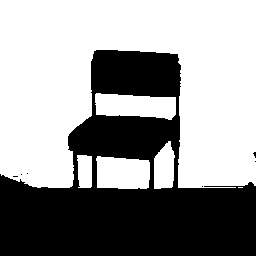
\includegraphics[width=0.2\textwidth]{img/res/e1a/alg1tipo1-chair.jpg} &
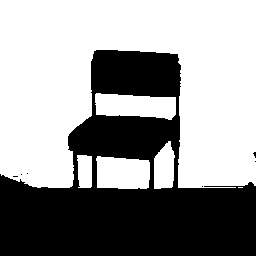
\includegraphics[width=0.2\textwidth]{img/res/e1a/alg1tipo6-chair.jpg} &
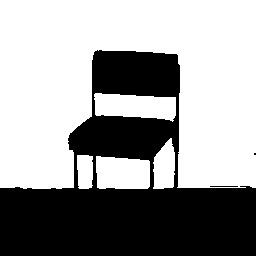
\includegraphics[width=0.2\textwidth]{img/res/e1a/alg1tipo6d0.75-chair.jpg} &
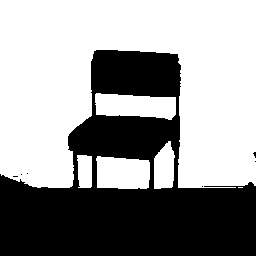
\includegraphics[width=0.2\textwidth]{img/res/e1a/alg1tipo6d1.25-chair.jpg} \\
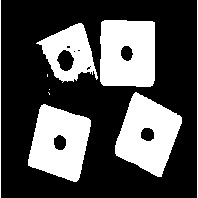
\includegraphics[width=0.2\textwidth]{img/res/e1a/alg1tipo1-block.jpg} &
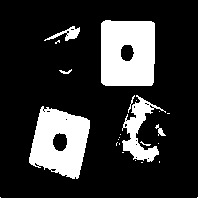
\includegraphics[width=0.2\textwidth]{img/res/e1a/alg1tipo6-block.jpg} &
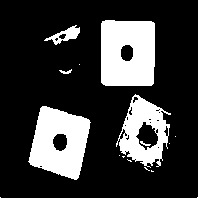
\includegraphics[width=0.2\textwidth]{img/res/e1a/alg1tipo6d0.75-block.jpg} &
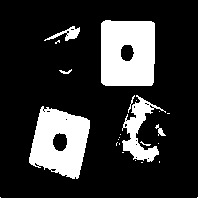
\includegraphics[width=0.2\textwidth]{img/res/e1a/alg1tipo6d1.25-block.jpg} \\
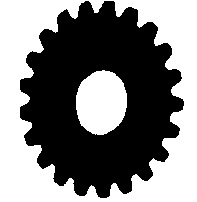
\includegraphics[width=0.2\textwidth]{img/res/e1a/alg1tipo1-02.jpg} &
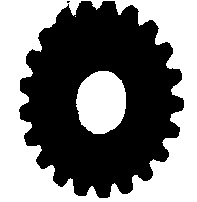
\includegraphics[width=0.2\textwidth]{img/res/e1a/alg1tipo6-02.jpg} &
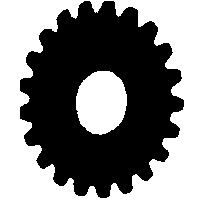
\includegraphics[width=0.2\textwidth]{img/res/e1a/alg1tipo6d0.75-02.jpg} &
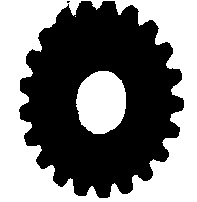
\includegraphics[width=0.2\textwidth]{img/res/e1a/alg1tipo6d1.25-02.jpg} \\
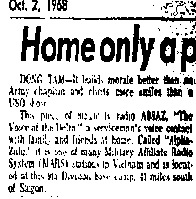
\includegraphics[width=0.2\textwidth]{img/res/e1a/alg1tipo1-09.jpg} &
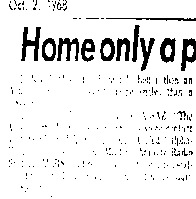
\includegraphics[width=0.2\textwidth]{img/res/e1a/alg1tipo6-09.jpg} &
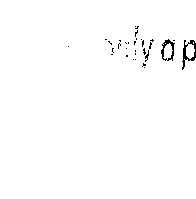
\includegraphics[width=0.2\textwidth]{img/res/e1a/alg1tipo6d0.75-09.jpg} &
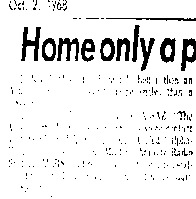
\includegraphics[width=0.2\textwidth]{img/res/e1a/alg1tipo6d1.25-09.jpg} \\
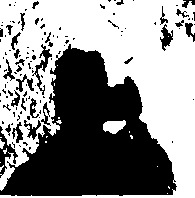
\includegraphics[width=0.2\textwidth]{img/res/e1a/alg1tipo1-07.jpg} &
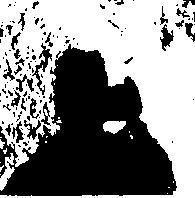
\includegraphics[width=0.2\textwidth]{img/res/e1a/alg1tipo6-07.jpg} &
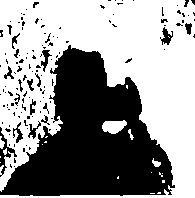
\includegraphics[width=0.2\textwidth]{img/res/e1a/alg1tipo6d0.75-07.jpg} &
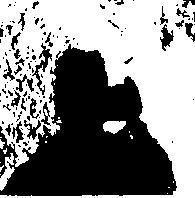
\includegraphics[width=0.2\textwidth]{img/res/e1a/alg1tipo6d1.25-07.jpg} \\\hline
\end{tabular}
\caption{Umbrales para las imágenes con ruido con otras versiones de algoritmos.\label{tab:resultexp1imagenesdombi}}
\end{table}


\begin{table}
\centering
\begin{tabular}{c||c|c|c} 
$\mathbf{REF_1=1-\abs{x-y}}$ & $\mathbf{w=0,75}$ &\bb $\mathbf{w=1}$ &\bb $\mathbf{w=1,25}$\\\hline\hline
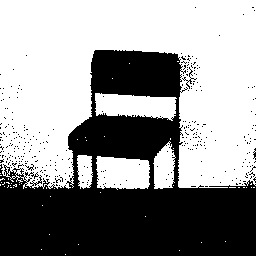
\includegraphics[width=0.2\textwidth]{img/res/e1a/alg1tipo1-chairga.jpg} &
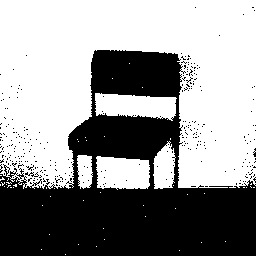
\includegraphics[width=0.2\textwidth]{img/res/e1a/alg1tipo6-chairga.jpg} &
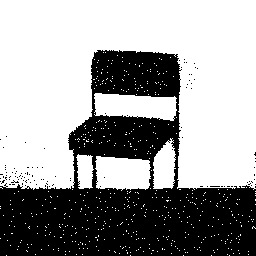
\includegraphics[width=0.2\textwidth]{img/res/e1a/alg1tipo6d0.75-chairga.jpg} &
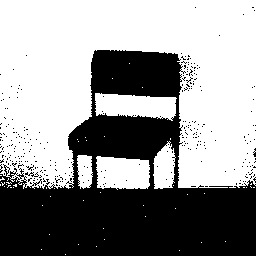
\includegraphics[width=0.2\textwidth]{img/res/e1a/alg1tipo6d1.25-chairga.jpg} \\
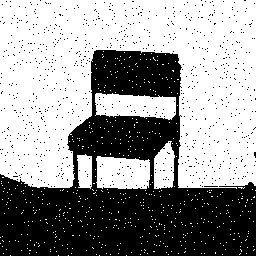
\includegraphics[width=0.2\textwidth]{img/res/e1a/alg1tipo1-chairsp005.jpg} &
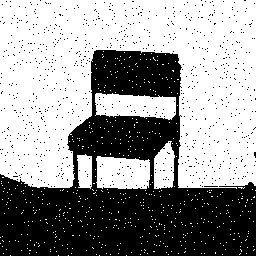
\includegraphics[width=0.2\textwidth]{img/res/e1a/alg1tipo6-chairsp005.jpg} &
\includegraphics[width=0.2\textwidth]{img/res/e1a/alg1tipo6d0.75-chairsp005.jpg} &
\includegraphics[width=0.2\textwidth]{img/res/e1a/alg1tipo6d1.25-chairsp005.jpg} \\
\includegraphics[width=0.2\textwidth]{img/res/e1a/alg1tipo1-chairsp020.jpg} &
\includegraphics[width=0.2\textwidth]{img/res/e1a/alg1tipo6-chairsp020.jpg} &
\includegraphics[width=0.2\textwidth]{img/res/e1a/alg1tipo6d0.75-chairsp020.jpg} &
\includegraphics[width=0.2\textwidth]{img/res/e1a/alg1tipo6d1.25-chairsp020.jpg} \\\hline
\end{tabular}
\caption{Umbrales para las imágenes con ruido con otras versiones de algoritmos.\label{tab:resultexp1imagenesruido}}
\end{table}


\begin{table}
\centering
\begin{tabular}{c||c|c|c|c} 
$\mathbf{w}$                    &\bb Bloques&\bb Engranaje&\bb Letras&\bb Sombra\\\hline\hline
\bb Alg. 1 con $\mathbf{0,75}$  &     &   0,0338   &   0,0291   &   0,1017  \\\hline
\bb Alg. 1 con $\mathbf{1}$     &     &   0,0213   &   0,0025   &   0,0650  \\\hline
\bb Alg. 1 con $\mathbf{1,25}$  &     &   0,0153   &   0,0001   &   0,0322  \\\hline
\end{tabular}
\caption{Errores para las imágenes con ruido con otras versiones de algoritmos.\label{tab:erroresexp1dombi}}
\end{table}

\REV{Los errores de las imágenes con ruido son 0}



% EXPERIMENTO 2
\subsection{Experimento 2: busqueda del mejor umbral a través de funciones penalti}
\subsubsection{Explicación del experimento}
En vista del experimento anteior donde había momentos en los que la función de dombi no actuaba de forma correcta, se propone una nueva forma para poder elegir entre la función de Dombi o volver al método con la función REF. En concreto, se intentará dilucidar esta situación por medio de una función penalti. El proceso de la obtención del conjunto difuso cambiará, ya que no será una única función y tendrá un orden similar al siguiente:
\begin{itemize}
    \item Creación de todas las pertenencias con las 5 funciones REF presentadas y Dombi?
    \item Agregación de todas las pertenencias anteriores con varias funciones, a saber:
        \begin{enumerate}
            \item Media aritmética.
            \item Media geométrica.
            \item Máximo.
            \item Mínimo.
            \item Integral Choquet.
            \item OWA de la mayoría. \REV{nombre}
        \end{enumerate}    
    \item Con todos estos resultados se actua con la función penalti para cada uno de los elementos $a_1,\dots a_n$ agregados y las pertenencias obtenidas en (1) $r_1,\dots, r_m$, obtendremos $p(a_i, r)=\sum_{j=1}^m \abs{a_i-r_j}$.
    \item Cogeremos como pertenencia aquel resultado de la agregación, $a_i$, que haga que el resultado de la función penalti sea máximo.  
\end{itemize}

En una segunda versión, se añadirá también la función de agregación 
$$M_{zadeh}(r_1,\dots,r_m)=\max\left(0, \sum r-(n-1)\right)\cdot \sqrt[n]{\prod_{i=1}^n{r_i}}$$

\subsubsection{Resultados}

\begin{table}
\centering
\begin{tabular}{c||c|c|c|c|c} 
                &\bb Silla&\bb Bloques&\bb Engranaje&\bb Letras&\bb Sombra\\\hline\hline
$\mathbf{w=1}$  &   127   &     68    &      92     &   196    &   123  \\\hline
\end{tabular}
\caption{Umbrales para cada imagen con el algoritmo 1 calculando la función de pertenencia a través de una función penalti.\label{tab:resultexp1dombiagregado}}
\end{table}
Tiempo igual a 0,0023 s.

\begin{table}
\centering
\begin{tabular}{c||c|c|c} 
                          &\bb R. gausiano&\bb R. impulsivo 0.05&\bb R. impulsivo 0.2\\\hline\hline
\bb Alg. 1 con $\mathbf{REF_1=1-\abs{x-y}}$             &   132   &    127    &     127     \\\hline
\bb Alg. 1 con $\mathbf{REF_1=1-\abs{x-y}^2}$           &   131   &    127    &     127     \\\hline
\bb Alg. 1 con $\mathbf{REF_1=1-\abs{x-y}^{0.5}}$       &   131   &    136    &     152     \\\hline
\bb Alg. 1 con $\mathbf{REF_1=(1-\abs{x-y})^2}$         &   132   &    127    &     127     \\\hline
\bb Alg. 1 con $\mathbf{REF_1=(1-\abs{x-y})^{0.5}}$     &   131   &    127    &     127     \\\hline
\bb U. Global                                           &   132   &    130    &     128     \\\hline
\bb U. de Otsu                                          &   132   &    123    &     123     \\\hline
\bb Máx. la entropía de Renyi                           &   154   &    170    &     170     \\\hline
\end{tabular}
\caption{Umbrales para las imágenes con ruido con otras versiones de algoritmos.\label{tab:resultexp1ruidootros}}
\end{table}


\begin{table}
\centering
\begin{tabular}{ccccc}\hline
\includegraphics[width=0.15\textwidth]{img/res/e2a/alg1agregate-chair.jpg} &
\includegraphics[width=0.15\textwidth]{img/res/e2a/alg1agregate-block.jpg} &
\includegraphics[width=0.15\textwidth]{img/res/e2a/alg1agregate-02.jpg} &
\includegraphics[width=0.15\textwidth]{img/res/e2a/alg1agregate-09.jpg} &
\includegraphics[width=0.15\textwidth]{img/res/e2a/alg1agregate-07.jpg}\\\hline
\end{tabular}
\caption{Resultado para el nuevo algoritmo a través de penalti con todas las funciones propuestas.\label{tab:resultexp2agregado}}
\end{table}



\begin{table}
\centering
\begin{tabular}{ccc}\hline
\includegraphics[width=0.15\textwidth]{img/res/e2a/alg1agregate-chairga.jpg} &
\includegraphics[width=0.15\textwidth]{img/res/e2a/alg1agregate-chairsp005.jpg} &
\includegraphics[width=0.15\textwidth]{img/res/e2a/alg1agregate-chairsp020.jpg}\\\hline
\end{tabular}
\caption{Resultado para el nuevo algoritmo a través de penalti con todas las funciones propuestas para imágenes con ruido.\label{tab:resultexp2agregado}}
\end{table}

\REV{Calcular los errores }


% EXPERIMENTO 3
\subsection{Experimento 3: sustitución de la función REF por la función de Dombi en el algoritmo para la obtenición del umbral óptimo}

\subsubsection{Explicación del experimento}
En este experimento se ha tomado el algoritmo de obtención del umbal óptimo maximizando la similitud para comprobar el efecto de la función de Dombi en él. Por esta razón, y en vista de los resultados del experimento 1, se plantean dos variantes. En primer lugar, se incorpora la función de dombi a las 5 funciones REF que ya estaban para poder ver qué umbral se obtiene. Después, se eligen los diferentes valores de $w$ que se han utilizado antes. De esta forma, se intenta buscar cual de los umbrales calculados anteriormente de forma individual es el mejor.

\subsubsection{Resultados}
\begin{table}
\centering
%\resizebox*{3\textwidth}{!}{
\begin{tabular}{c||c|c|c|c|c} 
             &\bb Silla&\bb Bloques&\bb Engranaje&\bb Letras&\bb Sombra\\\hline\hline
\bb Alg. 3A  &    50   &    119    &     88      &    199   &    121   \\\hline
\bb Alg. 3B  &   123   &    127    &     84      &    200   &    125   \\\hline
\bb Alg. 3C  &   254   &    218    &     250     &    142   &    219   \\\hline
\end{tabular}
\caption{Umbrales para cada imagen con el algoritmo 3 en todas sus versiones.\label{tab:resultexp3dombi}}
\end{table}


\subsubsection{Resultados}
\begin{table}
\centering
%\resizebox*{3\textwidth}{!}{
\begin{tabular}{c||c|c|c}
        &\bb R. gausiano&\bb R. impulsivo 0.05&\bb R. impulsivo 0.2\\\hline\hline
\bb Alg. 3A  &   131   &    136    &     144      \\\hline
\bb Alg. 3B  &   128   &    127    &     127      \\\hline
\bb Alg. 3C  &   226   &    218    &     226      \\\hline
\end{tabular}
\caption{Umbrales para cada imagen con el algoritmo 3 en todas sus versiones.\label{tab:resultexp3dombi}}
\end{table}


\begin{table}
\centering
\begin{tabular}{cccccc}\hline
Alg. 3B\quad
\includegraphics[width=0.15\textwidth]{img/res/e3a/alg3btipo-chair.jpg} &
\includegraphics[width=0.15\textwidth]{img/res/e3a/alg3btipo-block.jpg} &
\includegraphics[width=0.15\textwidth]{img/res/e3a/alg3btipo-02.jpg} &
\includegraphics[width=0.15\textwidth]{img/res/e3a/alg3btipo-09.jpg} &
\includegraphics[width=0.15\textwidth]{img/res/e3a/alg3btipo-07.jpg}\\\hline
Alg. 3C\quad     
\includegraphics[width=0.15\textwidth]{img/res/e3a/alg3ctipo-chair.jpg} &
\includegraphics[width=0.15\textwidth]{img/res/e3a/alg3ctipo-block.jpg} &
\includegraphics[width=0.15\textwidth]{img/res/e3a/alg3ctipo-02.jpg} &
\includegraphics[width=0.15\textwidth]{img/res/e3a/alg3ctipo-09.jpg} &
\includegraphics[width=0.15\textwidth]{img/res/e3a/alg3ctipo-07.jpg}\\\hline
\end{tabular}
\caption{Resultado para el nuevo algoritmo a través de penalti con todas las funciones propuestas.\label{tab:resultexp3imagenesdombi}}
\end{table}


\begin{table}
\centering
\begin{tabular}{c||c|c|c|c}
                &\bb Bloques  &\bb Engranaje&\bb Letras  &\bb Sombra  \\\hline\hline
\bb Alg. 3B     &   \REV{revisar}   &   0,01236   &   0,2019   &   0,1017   \\\hline
\bb Alg. 3C     &      &   0,50552   &   0,0136   &   0,5744   \\\hline
\end{tabular}
\caption{Umbrales para cada imagen con el algoritmo 3 en todas sus versiones.\label{tab:erroresexp3dombi}}
\end{table}


\begin{table}
\centering
\begin{tabular}{c||c|c|c|c}
                        &\bb Silla    &\bb Bloques  &\bb Engranaje &\bb Sombra    \\\hline\hline
\bb Alg. 3 Original     &   72,8822   &   93,8135   &   126,5836   &   124,7987   \\\hline
\bb Umb. Global         &   71,7070   &   81,0453   &   124,7637   &   122,4343   \\\hline
\bb {\em K-means}       &   71,7070   &   81,0453   &   124,9112   &   123,2863   \\\hline
\bb Método de Otsu      &   71,7070   &   81,0453   &   124,9112   &   123,2863   \\\hline
\bb Máx. Entropía Renyi &   56,9290   &   96,4543   &   121,5597   &   112,4747   \\\hline
\end{tabular}
\caption{Umbrales para cada imagen con el algoritmo 3 en todas sus versiones.\label{tab:erroresexp3otros}}
\end{table}


\begin{table}
\centering
\begin{tabular}{cccccc}\hline
Alg. 3B\quad
\includegraphics[width=0.18\textwidth]{img/res/e3a/alg3btipo-chairga.jpg} &
\includegraphics[width=0.18\textwidth]{img/res/e3a/alg3btipo-chairsp005.jpg} &
\includegraphics[width=0.18\textwidth]{img/res/e3a/alg3btipo-chairsp020.jpg}\\\hline
Alg. 3C\quad     
\includegraphics[width=0.18\textwidth]{img/res/e3a/alg3ctipo-chairga.jpg} &
\includegraphics[width=0.18\textwidth]{img/res/e3a/alg3ctipo-chairsp005.jpg} &
\includegraphics[width=0.18\textwidth]{img/res/e3a/alg3ctipo-chairsp020.jpg}\\\hline
\end{tabular}
\caption{Resultado para el nuevo algoritmo a través de penalti con todas las funciones propuestas.\label{tab:resultexp3imagenesdombi}}
\end{table}


\begin{table}
\centering
\begin{tabular}{c||c|c|c}
        &\bb R. gausiano&\bb R. impulsivo 0.05&\bb R. impulsivo 0.2\\\hline\hline
\bb Alg. 3 Original     &   95,1075   &   66,4737   &   74,2907   \\\hline
\bb Umb. Global         &   94,8740   &   68,2635   &   77,5124   \\\hline
\bb {\em K-means}       &   95,1074   &   68,2635   &   77,5124   \\\hline
\bb Método de Otsu      &   94,8740   &   68,2635   &   77,5124   \\\hline
\bb Máx. Entropía Renyi &   85,9364   &   54,1976   &   65,7772   \\\hline
\end{tabular}
\caption{Umbrales para cada imagen con el algoritmo 3 en todas sus versiones.\label{tab:erroresexp3ruido}}
\end{table}


\subsection{Repetición de los experimentos con la corrección oportuna.}
Como se ha explicado en el apartado anterior, sorprende la forma que toma ...
\begin{equation}
    \mu_{Q_t}(q)=\left\{ \begin{split}
                 \min\left( 1, \frac
                    {\unmedio \left(1+\left(1-\frac{2q}{L-1}\right)\left(1-\frac{2m_b}{L-1}\right)\right)}
                    {\unmedio \left(1+\left(1-\frac{2m_b}{L-1}\right)\left(1-\frac{2m_b}{L-1}\right)\right)}\right)
                 \text{\quad si\quad} q\leq t\\
                 \min\left( 1, \frac
                    {\unmedio \left(1+\left(1-\frac{2q}{L-1}\right)\left(1-\frac{2m_o}{L-1}\right)\right)}
                    {\unmedio \left(1+\left(1-\frac{2m_o}{L-1}\right)\left(1-\frac{2m_o}{L-1}\right)\right)}\right)
                \text{\quad si\quad} q > t
                \end{split}\right.
\end{equation}



%RESULTADOS DE LA REESCRITURA

\begin{table}\begin{center}
%\resizebox*{3\textwidth}{!}{
\begin{tabular}{cc||c|c|c|c|c} 
                                    &                   &\bb Silla&\bb Bloques&\bb Engranaje&\bb Letras&\bb Sombra\\\hline\hline
\bb{\multirow{2}{1.75cm}{$w=0,1$}}  &  \bb Umbral ($t$) &   234   &     8     &      0      &   157    &   250  \\
                                    &  \bb Tiempo (s)   &  0,002  &   0,675   &    0,686    &  0,689   &  0,688 \\\hline
\bb\multirow{2}{1.75cm}{$w=0,5$}    &  \bb Umbral ($t$) &   226   &     8     &     111     &   207    &   254  \\
                                    &  \bb Tiempo (s)   &  0,002  &   0,649   &    1,093    &  1,233   &  1,13  \\\hline
\bb\multirow{2}{1.75cm}{$w=0,75$}   &  \bb Umbral ($t$) &   226   &     8     &     122     &   182    &   238  \\
                                    &  \bb Tiempo (s)   &  0,002  &   0,677   &    0,686    &  0,688   &  0,679 \\\hline
\bb\multirow{2}{1.75cm}{$w=1$}      &  \bb Umbral ($t$) &   226   &     8     &      90     &   191    &   246  \\
                                    &  \bb Tiempo (s)   &  0,002  &   0,63    &    0,642    &  0,646   &  0,642 \\\hline
\bb\multirow{2}{1.75cm}{$w=1,25$}   &  \bb Umbral ($t$) &   226   &     8     &     250     &   203    &   252  \\
                                    &  \bb Tiempo (s)   &  0,002  &   0,682   &    0,684    &  0,688   &  0,686 \\\hline
\bb\multirow{2}{1.75cm}{$w=1,5$}    &  \bb Umbral ($t$) &   242   &     6     &     250     &   213    &   254  \\
                                    &  \bb Tiempo (s)   &  0,002  &   0,666   &    1,106    &  1,246   &  1,138 \\\hline
\bb\multirow{2}{1.75cm}{$w=2$}      &  \bb Umbral ($t$) &   250   &     3     &     250     &   215    &    66  \\
                                    &  \bb Tiempo (s)   &  0,002  &   0,631   &    0,640    &  0,644   &  0,641 \\\hline
\bb\multirow{2}{1.75cm}{$w=5$}      &  \bb Umbral ($t$) &   250   &     1     &     250     &   254    &    66  \\
                                    &  \bb Tiempo (s)   &  0,002  &   0,657   &    0,671    &  0,672   &  0,673 \\\hline
\end{tabular}\end{center}
\caption{Umbrales y tiempo de cómputo para cada imagen con funciones de Dombi reescrita.\label{tab:resultexp1dombi}}
\end{table}

\begin{table}\begin{center}
%\resizebox*{3\textwidth}{!}{
\begin{tabular}{cc||c|c|c} 
                                   &           &\bb Ruido gausiano&\bb Ruido impulsivo 0.05&\bb Ruido impulsivo 0.2\\\hline\hline
\bb\multirow{2}{1.75cm}{Alg. 3A}   &  \bb Umbral ($t$) &   131   &    136    &     144     \\
                                   &  \bb Tiempo (s)   &  0,002  &   0,002   &    0,002    \\\hline
\bb\multirow{2}{1.75cm}{Alg. 3B}   &  \bb Umbral ($t$) &   131   &    234    &     152     \\
                                   &  \bb Tiempo (s)   &  0,002  &   0,002   &    0,002    \\\hline
\bb\multirow{2}{1.75cm}{Alg. 3C}   &  \bb Umbral ($t$) &   254   &    234    &     250     \\
                                   &  \bb Tiempo (s)   &  0,002  &   0,002   &    0,002    \\\hline
\end{tabular}\end{center}
\caption{Umbrales y tiempo de cómputo para cada imagen con funciones de Dombi reescrita.\label{tab:resultexp1dombi}}
\end{table}